\section{信息在流中的传递}
\subsection*{什么是流?}
程序与外界的一切交互都是依靠字符的\textbf{输入(Input)}和\textbf{输出(Output)}完成的。我们可以想像一条流水线,我们的输入字符从输入设备——比如键盘中产生,经过流水线,一个个地被程序接收。这就是\textbf{流(Stream)}。\par
对于输出信息来说,它也有一条(其实不止)流水线。输出字符从程序中产生,经过这条流水线,就能一个个地被输出设备——比如显示器所接收。\par
\begin{figure}[htbp]
    \centering
    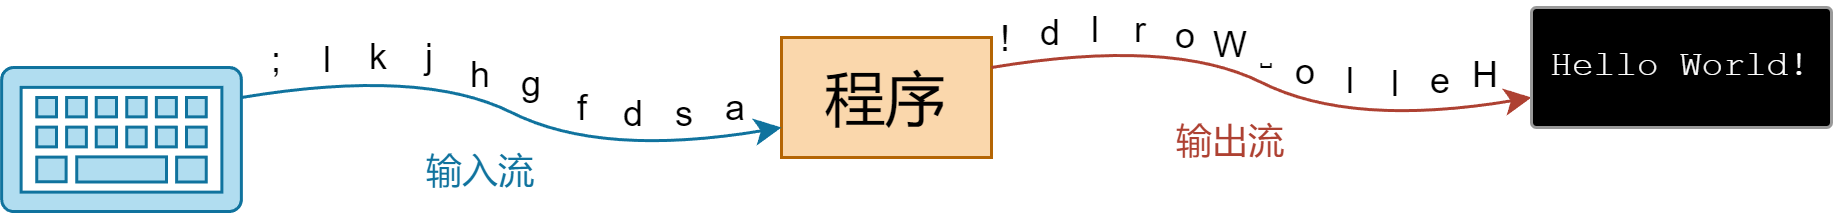
\includegraphics[width=\textwidth]{../images/generalized_parts/13_input_output_stream.drawio.png}
    \caption{程序的输入输出流}
    \footnotesize{仅供示意,输入内容与输出内容无因果关系}
\end{figure}
如图 \lstinline@13.2@所示,我们可以通过键盘输入一系列的内容到程序中,这时程序可以从输入流中逐个字符地读取我们的输入信息。程序还可以通过输出流把要输出的内容逐个字符地输出到相应的输出设备中,从而变成我们能在显示器中看到的信息。\par
总而言之,在流中传递的所有``信息'',都是以字符为单位的。所有的输入,都可以看作是字符输入;所有的输出,都可以看作是字符输出。当程序需要我们输入字符的时候,我们输入的是字符;当程序需要我们输入整数或者浮点数的时候,我们输入的也是字符。那么问题来了:程序要怎么把我们输入的``字符''变成保存在整型/浮点型变量中的``数''呢?这就要依靠 \lstinline@std::basic_istream@ 类模板中定义的重载运算符 \lstinline@>>@ 了。\par
\lstinline@std::basic_istream@ 提供了一套方法,这样就允许我们从输入流的若干字符当中整理出有效信息,并把这个值赋给对应的变量或对象。与 \lstinline@std::basic_istream@ 相关的 \lstinline@>>@ 运算符有很多重载,以下是其中的一部分,包括成员函数和非成员函数:
\begin{lstlisting}
basic_istream& basic_istream::operator>>(int &value); //向int变量中输入
//还有大量关于有符号/无符号的各种整型的重载
basic_istream& basic_istream::operator>>(double &value);
//还有关于float和long double的重载
template< class CharT, class Traits>
basic_istream<CharT, Traits>& operator>>(
    basic_istream<CharT, Traits> &st,
    CharT *s
); //向字符串中输入;也有CharT&的重载,可以向字符中输入
template< class CharT, class Traits, class Allocator >
std::basic_istream<CharT, Traits>& operator>>(
    std::basic_istream<CharT, Traits> &is,
    std::basic_string<CharT, Traits, Allocator> &str
); //向string对象中输入
\end{lstlisting}
假如我们要输入一个 \lstinline@int@ 型变量的值,那么程序就会调用 \lstinline@std::basic_istream::operator>>(int&)@。这个函数可以把读取到的字符信息提取(Extract)出来,从而赋值给对应的变量,这样就完成了一个输入操作。\par
同样的道理,当我们需要输出一个什么内容的时候,\lstinline@std::basic_ostream@ 相关的 \lstinline@<<@ 运算符重载就可以根据对应的类型,把整型或者浮点型或者其它类型的数据全都变成字符来输出。\par
\subsection*{输入源/输出目标与重定向}
对于一个流来说,字符信息从哪里来,哪里就是它的源(Source);字符信息要到哪里去,哪里就是它的目标(Target)。对于标准输入输出来说,程序输入流的源就是键盘,目标就是程序本身;程序输出流的源就是程序本身,目标就是显示器。\par
C语言来说有三种标准输入/输出——\lstinline@stdin@, \lstinline@stdout@, \lstinline@stderr@,分别表示标准输入、标准输出和标准错误输出。而C++是兼容C语言的。C++来说在 \lstinline@std@ 命名空间中定义了八个标准输入/输出流对象,我们用 \lstinline@#include<iostream>@ 即可包含它们。这八个对象可以对应到C语言的三种标准输入/输出。
\begin{itemize}
    \item \lstinline@std::cin@ 和 \lstinline@std::wcin@ 用于控制标准输入,对应C语言中的 \lstinline@stdin@;
    \item \lstinline@std::cout@ 和 \lstinline@std::wcout@ 用于控制标准输出,对应C语言中的 \lstinline@stdout@;
    \item \lstinline@std::clog@, \lstinline@std::cerr@, \lstinline@std::wclog@ 和 \lstinline@std::wcerr@ 用于控制标准错误输出,对应C语言中的 \lstinline@stderr@。
\end{itemize}
这八个对象中,带 \lstinline@w@ 前缀的四个表示宽字符输入/输出。我们目前不用也不讲。而 \lstinline@std::clog@ 与 \lstinline@std::cerr@ 的区别在于前者是带有缓冲区的,而后者没有。我们稍后来介绍缓冲区机制。\par
有些时候,我们会需要改变输入的源,或者改变输出的目标。我们可能需要从某个文件中读入信息,或者向某个文件中写入错误日志(这就可以用 \lstinline@std::clog@ 了)。C语言提供 \lstinline@freopen@ 之类的语法来允许我们进行\textbf{重定向(Redirection)},也就是改变源或者目标的位置。在C++中,我们可以通过 \lstinline@rdbuf@ 等成员函数来进行重定向。具体内容就留待精讲篇再介绍吧。\par
\subsection*{缓冲区}
在进行文件操作的时候,一个程序可能会频繁地从文件中不断读取少量的信息(比如一个不超过10字符长度的整数),然后自顾自地去进行下一步操作;过一会儿它又来了,又是读取一点点信息就走了。这种挤牙膏式的数据存取并不经济,因为外存或许能够一次性通过这个流传输1024字节(甚至更多)的数据,但我们却要分成几十上百次来完成,那么效率低也就不奇怪了\footnote{程序访问外存(文件中的信息存储于此)的速度要比访问内存(程序数据通常存储于此)的速度慢得多,我们在第一章中就提及过了。}。\par
为了提高效率,输入/输出一般会使用\textbf{缓冲区(Buffer)}。缓冲区是程序在内存中分配的的一段临时使用区域。当程序从外界(尤其是外存中的文件)读取内容时,它充分利用这一次读取的机会,一次性读取尽可能多的内容。那些尚不需要的内容会被储存在缓冲区中。等到下次输入时,程序就不需要从外界获取信息了,而是直接从缓冲区(在内存中)获取,这样效率就高了。\par
打个比方,你有一个小号的水杯。为了喝水,你必须频繁地去外面的水房打水。而缓冲区就像一个水壶,你可以去水房用水壶一次性多接点水。然后当你想要喝水时,你就可以从手边的水壶里直接倒出水来,不用总是拿着杯子去外面接水了。\par
输出缓冲区也是一样的道理,程序可以先把要输出的内容缓存起来,然后再一次性输出到显示器或者文件当中。这就好像,我们有了一个垃圾桶之后就不用每次出门扔垃圾了,可以存一袋再一起扔。(这个比喻当然不是很恰当,输出内容可未必是垃圾)\par
但是有些时候,有些信息是不能缓存的,比如运行时的报错信息(异常信息)。如果使用缓冲区的话,就存在一种风险:程序通过 \lstinline@std::cout@ 输出了报错信息,但是报错信息还留在缓冲区里没出来,用户没看到,还继续一意孤行地在错误的道路上渐行渐远呢。\par
这个时候我们就应该使用 \lstinline@std::cerr@ 了。还记得我们上文怎么说的吗?这个对象是没有缓冲区的。没有缓冲区当然会导致挤牙膏一样的低效输出,但是——我们本来就不是为了用它输出正常信息的。什么时候我们可能用它呢?比如说,异常处理。
\begin{lstlisting}
    try {
        //...
    } catch (const std::exception &msg) {
        std::cerr << "An exception has been caught:\n" << msg.what();
    }
\end{lstlisting}
对于异常处理来说,使用 \lstinline@std::cerr@ 就不会存在缓冲区风险了。\par
如果我们有需要手动刷新输出缓冲区的话,可以调用 \lstinline@std::ostream@ 对象的 \lstinline@flush@ 成员函数。\par
如果我们还同时有换行需求的话,那么我们可以不用手动 \lstinline@flush@ 了,直接写一个 \lstinline@std::cout<<std::endl@ 就行。这个语句就意味着两个操作:输出一个换行符,然后顺便刷新缓冲区。\par
当然,这也就意味着,如果我们要进行文件操作之类的话,就要少用 \lstinline@std::endl@ 来换行了,应该尽可能使用 \lstinline@'\n'@ 这样的操作。否则就会不断刷新缓冲区,和挤牙膏没什么区别了。\par
